\chapter{Общие сведения о симуляторе LTspice. Базовые принципы работы}

\section{Установка симулятора LTspice}

Симулятор LTspice является бесплатпрограммым обеспечением, которое можно 
получить с официального сайта фирмы Analog Devices на странице загрузки по 
ссылке 
\href{
https://www.analog.com/ru/design-center/design-tools-and-calculators/ltspice-sim 
ulator.html}{
https://www.analog.com/ru/design-center/design-tools-and-calculators/ltspice-sim
}

\begin{figure}[H]
 \centering
 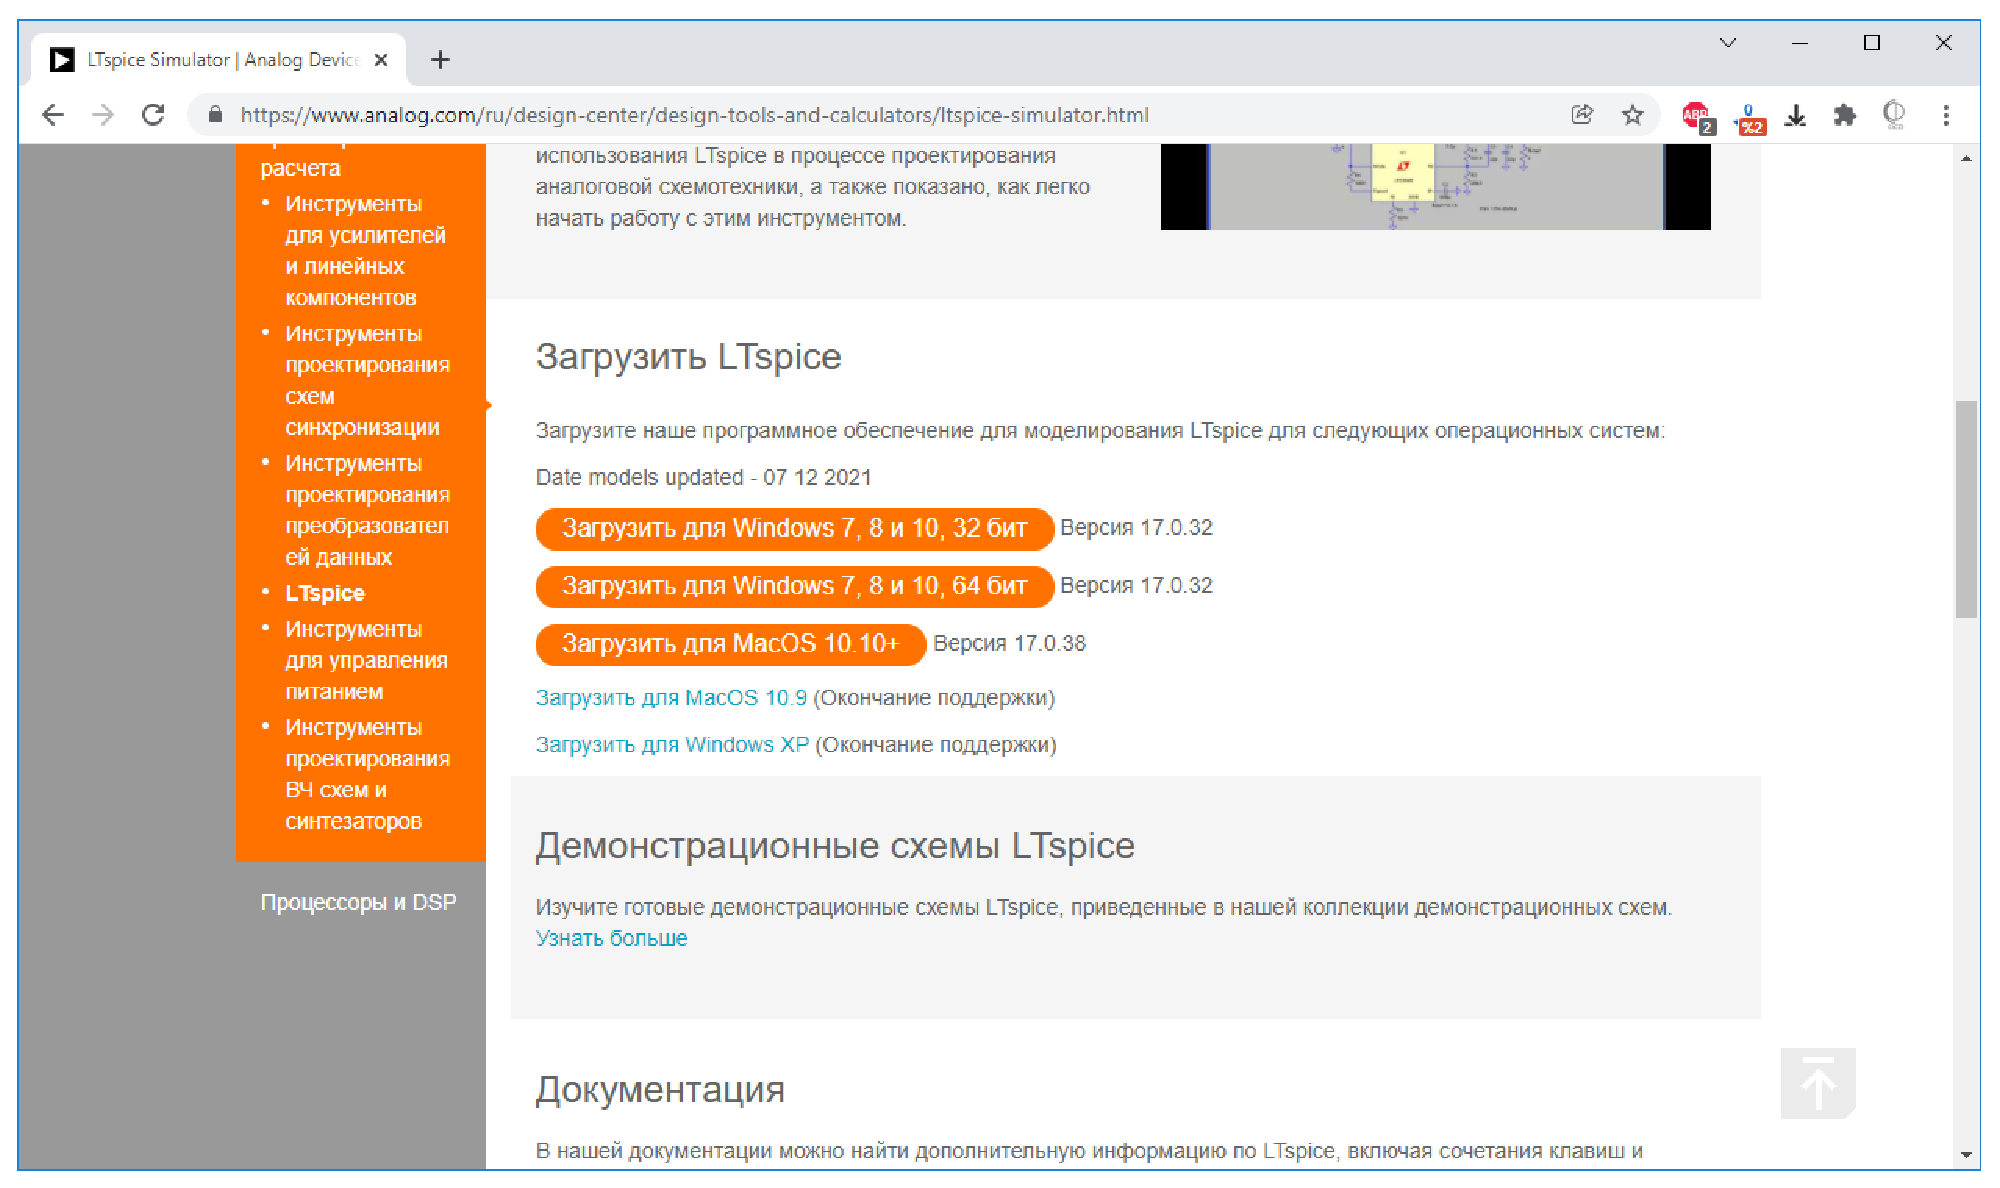
\includegraphics[width=0.7\textheight]{pic001.eps}
 \caption{Страница загрузки LTspice}
 \label{fig:download-page}
\end{figure}
На этой странице необходимо выбрать вариант загрузки для той операционной 
системы, которая установлена на вашем компьютере. Доступны варианты для OS 
Windows версий 7/8/10 разрядности 32 и 64 бит, вариант для операционной системы 
macOS, а так же вариант для Windows XP.

Скачав дистрибутив программы, необходимо установить его, способом, предлагаемым 
в вашей версии операционной системы.

При установке в OS Windows всех версий на рабочем столе появится ярлык для 
запуска симулятора.

\begin{figure}[H]
 \centering
 
\includegraphics[width=3cm]{pic002.eps}
 \caption{Ярлык для запуска LTspice на рабочем столе Windows}
 \label{fig:ltspice-icon}
\end{figure}

При первом запуске симулятор сформирует в домашнем каталоге пользователя 
каталоги с библиотеками электронных компонентов, на что потребуется некоторое 
время, 

\begin{figure}[H]
 \centering
 
\includegraphics[width=7cm]{unpack.eps}
 \caption{Инициализация библиотек LTspice}
 \label{fig:unpack}
\end{figure}
после чего появится главное рабочее окно LTspice

\begin{figure}[H]
 \centering
 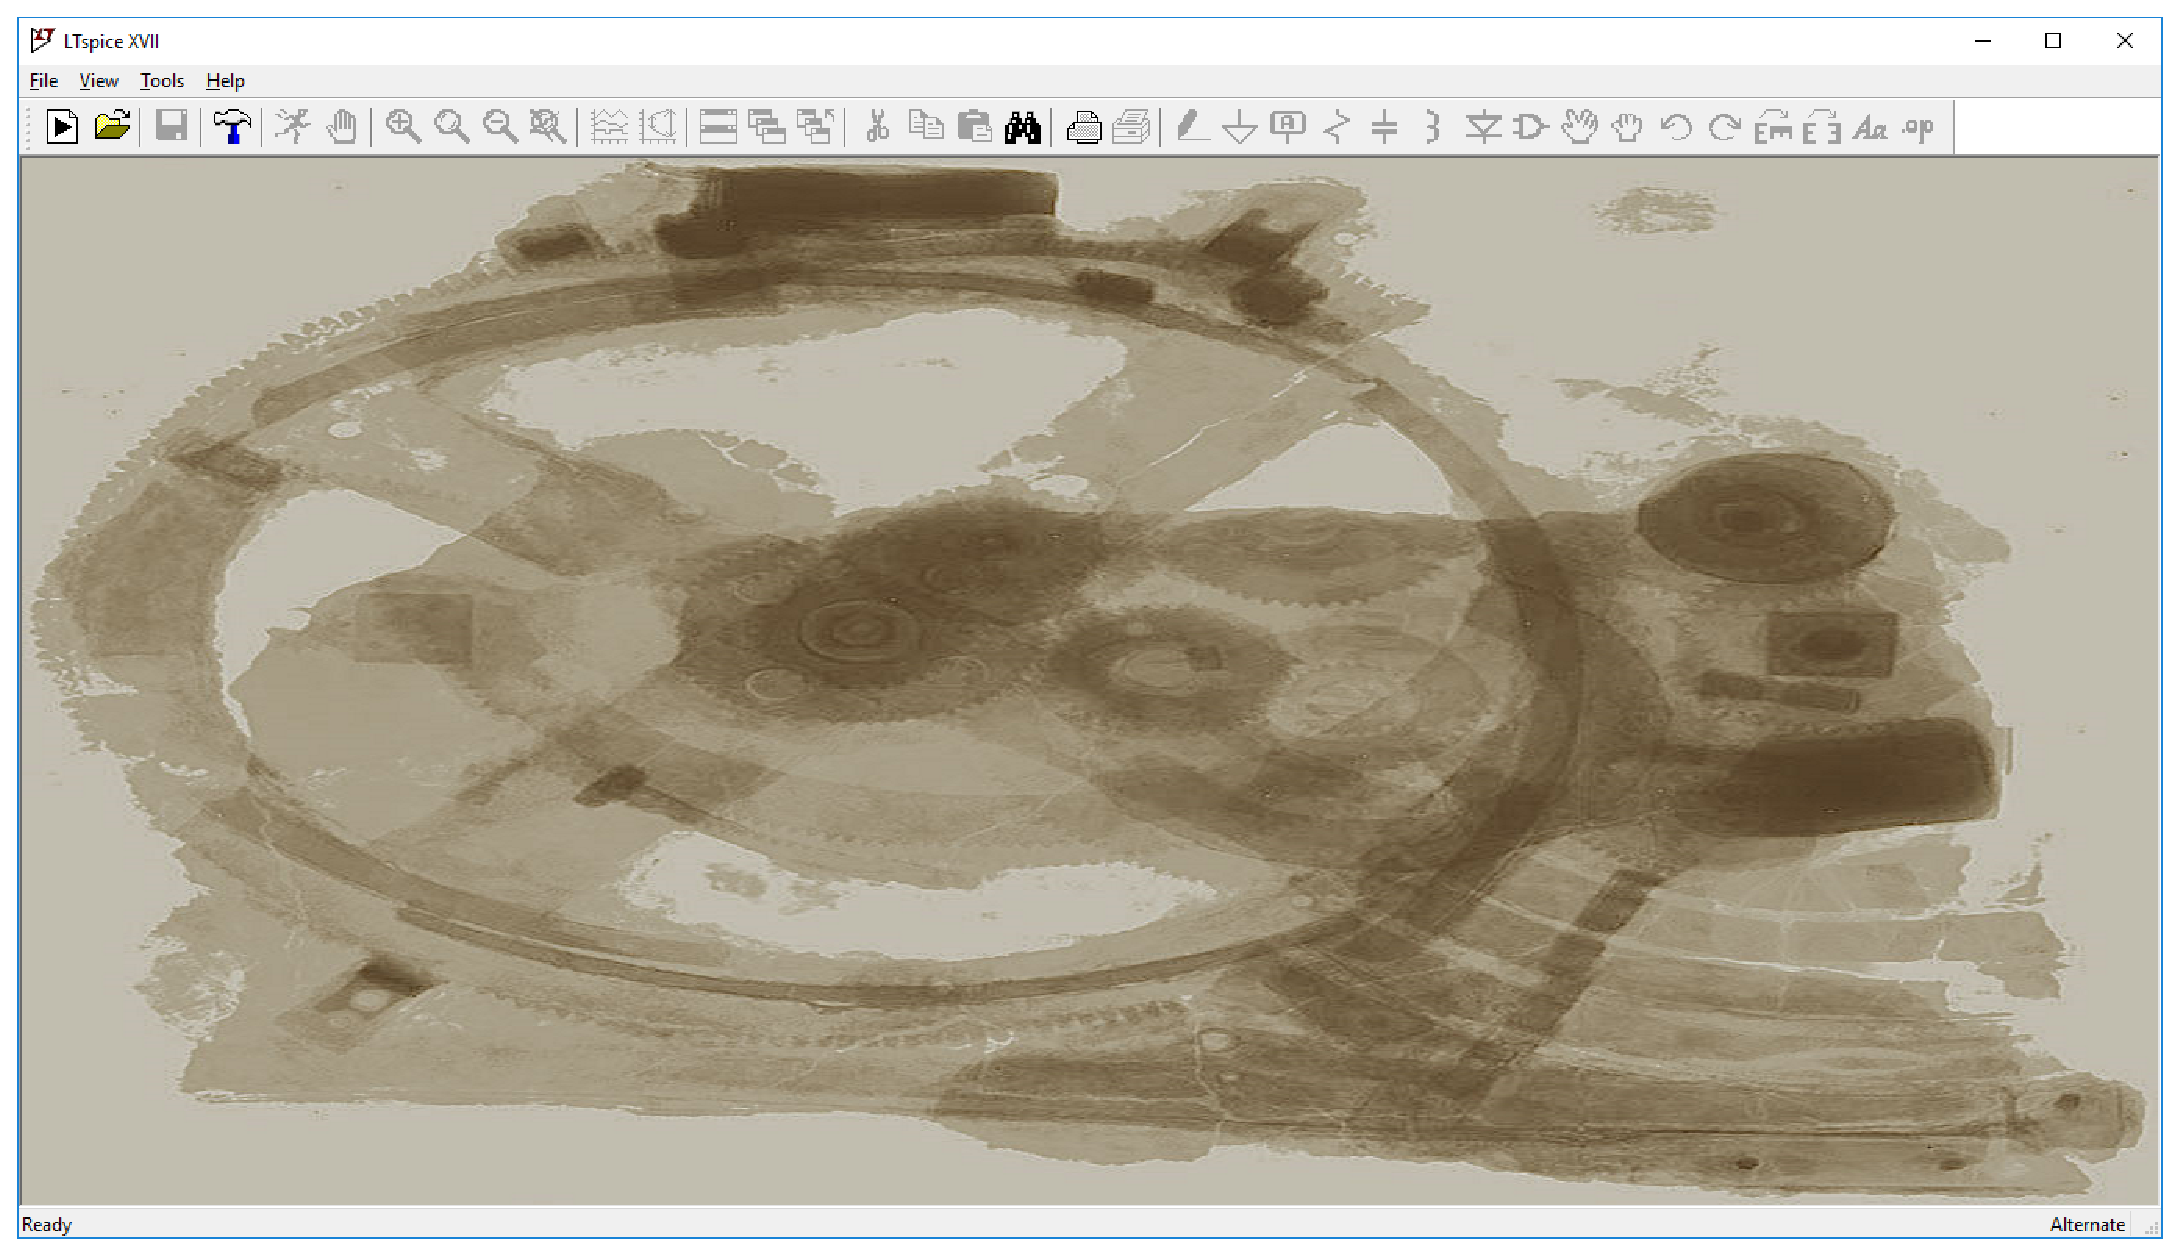
\includegraphics[width=17cm]{main-window.eps}
 \caption{Главное окно LTspice}
 \label{fig:main-window}
\end{figure}

Симулятор периодически обновляется разработчиками, поэтому, при последующих 
запусках может случится так, что вы увидете окно примерно такого вида

\begin{figure}[H]
 \centering
 
\includegraphics[width=10cm]{update-req.eps}
 \caption{Запрос обновления LTspice при запуске}
 \label{fig:update-req}
\end{figure}
Прошло некоторое время с установки симулятора на ваш 
компьютер, и программа проверяет наличие обновлений. Если ваш компьютер имеет 
доступ в Интернет, нажимаем <<Да>> и дожидаемся завершения обновления 
программы. В этом случае процесс обновления будет отображаться в таком окне

\begin{figure}[H]
 \centering
 
\includegraphics[width=17cm]{update-progress.eps}
 \caption{Окно прогресса обновления}
 \label{fig:update-progress}
\end{figure}
По окончании обновления симулятор сообщит об этом окном
\begin{figure}[H]
 \centering
 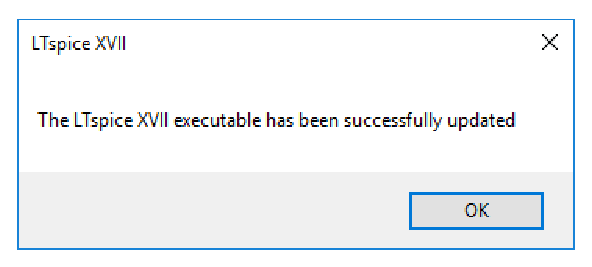
\includegraphics[width=10cm]{update-success.eps}
 \caption{Окно завершения обновления}
 \label{fig:update-success}
\end{figure}
на котором следует нажать <<Ок>> для перезапуска симулятора. Если вы, по камим либо причинам, не хотите 
ждать обновления, либо ваш компьютер не имеет доступа в сеть, нажмите <<Нет>> в окне на 
рисунке~\ref{fig:update-req}. Симулятор запустится в обычном режиме и некоторое 
время не будет запрашивать обновления.

